%========================================================
\chapter{Simulation Diagnostics: Baseline vs.\ Stable}
\label{chap:sim_comparison}
%========================================================

The previous chapter established that the baseline autoencoder satisfies the
theoretical conditions for existence and uniqueness of the latent SDE solution.
It also showed, in theory, why the baseline is \emph{not} guaranteed to produce
well-behaved simulated paths: the drift matrix $M$ can have positive eigenvalues
and the volatility network can output large values at states far from the training
cloud.
This chapter turns those theoretical warnings into a concrete empirical demonstration.

We simulate $N = 500$ paths over a 10-year horizon ($\Delta t = 1/12$, 120 monthly
steps) using both the baseline and stable checkpoints trained for 3\,500 epochs
($\ell = 2$, EUR swap curves).
\emph{Identical} Brownian increments are used for both models, so any difference
between the paths is attributable solely to the learned network parameters, not to
stochastic variation.
The figures and statistics below are generated by the script
\texttt{compare\_simulation\_variants.py}.


%========================================================
\section{Problems with the baseline model during simulation}
\label{sec:sim_baseline_problems}
%========================================================

Three distinct failure modes can arise when the baseline model is used for
forward simulation.  They are ordered by severity: the third (explosive drift)
is catastrophic and renders the model entirely unusable for pricing.

%--------------------------------------------------------
\subsection{Unstable drift: non-mean-reverting latent factors}
\label{subsec:unstable_drift}
%--------------------------------------------------------

The baseline drift network performs the affine map
\[
    \mathcal{K}(z) = Mz + N, \qquad M \in \mathbb{R}^{\ell \times \ell},
\]
where $M$ and $N$ are learned without any constraint on the eigenvalues of $M$.
As shown in Proposition~2 of Chapter~\ref{chap:stable_ae} (the Stable chapter),
mean reversion toward the fixed point $z^* = -M^{-1}N$ requires \emph{all}
eigenvalues of $M$ to have strictly negative real parts, i.e.\ $M$ must be
a \emph{Hurwitz} matrix.

When $M$ has at least one eigenvalue with non-negative real part, the
corresponding component of the deviation $u_t = z_t - z^*$ grows without bound
as $t \to \infty$.
In the Euler--Maruyama discretisation this means the latent state can drift
arbitrarily far from the training cloud within a finite simulation horizon.

\paragraph{What we observe in the ep3500 baseline.}
After 3\,500 training epochs, the baseline drift matrix has learned parameters
such that the latent paths explode within the 10-year window.
The console statistics from the simulation confirm this:
\begin{center}
\begin{tabular}{lrr}
\toprule
& \textbf{Baseline (ep3500)} & \textbf{Stable (ep3500)} \\
\midrule
$z_1$ mean  & $-6.3 \times 10^{16}$ & $-0.04$ \\
$z_1$ std   & $6.8 \times 10^{18}$  & $0.61$  \\
$z_1$ min   & $-5.9 \times 10^{20}$ & $-2.38$ \\
$z_1$ max   & $\phantom{-}1.4 \times 10^{20}$ & $\phantom{-}3.76$ \\
\midrule
$z_2$ mean  & $-5.8 \times 10^{16}$ & $-0.29$ \\
$z_2$ std   & $6.3 \times 10^{18}$  & $0.27$  \\
$z_2$ min   & $-5.4 \times 10^{20}$ & $-2.48$ \\
$z_2$ max   & $\phantom{-}1.3 \times 10^{20}$ & $\phantom{-}0.49$ \\
\bottomrule
\end{tabular}
\end{center}
The baseline latent state reaches values on the order of $10^{20}$, which is
roughly $10^{20}$ times larger than the training support ($|z| \lesssim 1$).
All paths have effectively diverged to floating-point extremes by the end of the
simulation window.

%--------------------------------------------------------
\subsection{Unbounded and unstable short rates}
\label{subsec:unstable_short_rate}
%--------------------------------------------------------

The short-rate network $\mathcal{R}(z)$ maps the latent state to a scalar via
a two-layer feedforward network with the centered soft-step activation
$\psi(x)=\sigma(x)-\tfrac{1}{2}\in(-\tfrac{1}{2},\tfrac{1}{2})$:
\[
    \tilde{r}(z)=W_2\,\psi(W_1 z),\qquad
    W_1\in\mathbb{R}^{h\times\ell},\;W_2\in\mathbb{R}^{1\times h},
\]
with no bias terms. Because $\psi$ is component-wise bounded in
$(-\tfrac{1}{2},\tfrac{1}{2})$, the output satisfies
$|\tilde{r}(z)|\leq\tfrac{1}{2}\|W_2\|_1$ for \emph{every} $z$.
This prevents the short rate itself from reaching infinity at any individual
time step.
However, once the latent state has diverged to $\|z\| \sim 10^{20}$, the
short-rate network is evaluated deep in its saturation regime: every path is
stuck at either $r_{\min}$ or $r_{\max}$, removing all cross-sectional and
time-series variation.

In the baseline simulation the short rate saturates at $\pm 114$\,bp with a
standard deviation of 109\,bp --- a bimodal distribution concentrated at the
network's hard limits rather than a plausible interest-rate distribution.
This makes any discount factor or derivative price computed from these paths
economically meaningless.

%--------------------------------------------------------
\subsection{Compound effect: simulation is unusable for pricing}
\label{subsec:compound_effect}
%--------------------------------------------------------

The two problems above interact multiplicatively.
Once the latent state escapes the training cloud, the decoder $\mathcal{G}$ is
evaluated at a wildly out-of-distribution input, producing bond prices and swap
rates that bear no relation to observed market data.
Crucially, this happens \emph{quickly}: Figure~\ref{fig:comp_latent_paths} shows
that even the individual path spaghetti plot is dominated by extreme values,
while the stable paths remain on a reasonable scale.

The conclusion is stark: a model that fits the training data perfectly but has an
unstable drift is \emph{entirely unsuitable} for simulation-based derivative pricing.
Reconstruction accuracy is a necessary but far from sufficient condition for a
pricing model.


%========================================================
\section{How the stable model solves each problem}
\label{sec:sim_stable_solutions}
%========================================================

The stable variant addresses each of the three failure modes through targeted
structural modifications, detailed in Chapter~\ref{chap:stable_ae}.
Here we summarise each fix and connect it to what we see in the figures.

%--------------------------------------------------------
\subsection{Fix 1: Guaranteed mean reversion via the Hurwitz constraint}
\label{subsec:fix_hurwitz}
%--------------------------------------------------------

The stable drift replaces the unconstrained matrix $M$ with
\[
    M = -\!\left(V^\top V + \varepsilon I_\ell\right), \qquad
    V \in \mathbb{R}^{\ell \times \ell}, \quad \varepsilon > 0.
\]
Since $V^\top V$ is positive semi-definite and $\varepsilon I$ is strictly positive
definite, the matrix $M$ is \emph{negative definite} for every choice of $V$.
All eigenvalues satisfy $\lambda_i \leq -\varepsilon < 0$, so the drift always
pulls $z_t$ back toward the equilibrium $z^* = -M^{-1}N$.

In the 10-year simulation, the stable latent factors revert to a neighbourhood
of $z^*$ and remain there throughout (Table above, right column;
Figures~\ref{fig:comp_fans} and~\ref{fig:comp_short_rate_fan}).
The paths spread naturally from the initial point and then stabilise,
exactly as a well-posed Ornstein--Uhlenbeck-type process should.

%--------------------------------------------------------
\subsection{Fix 2: Bounded volatilities via sigmoid link}
\label{subsec:fix_sigma}
%--------------------------------------------------------

The baseline volatility $\sigma_i(z) = \exp([\mathcal{H}(z)]_i)$ is bounded
theoretically by the network architecture, but the practical upper bound
$e^{C_{\mathrm{pre}}}$ can be large and is not controlled.
The stable network replaces the $\exp$-link with a sigmoid-bounded parameterization:
\[
    \log\sigma_i(z) = \log\sigma_{\min}
        + (\log\sigma_{\max} - \log\sigma_{\min})\cdot
          \operatorname{sigmoid}(h_i(z) + b_i),
\]
so that $\sigma_i(z) \in (\sigma_{\min}, \sigma_{\max})$ for \emph{every} $z$,
including states far outside the training cloud.
With default bounds $\sigma_{\min} = 10^{-4}$ and $\sigma_{\max} = 2.0$,
the diffusion can never produce a shock larger than $\sigma_{\max}\sqrt{\Delta t}$
per step, which prevents runaway path growth even if the drift were imperfect.

In combination with the Hurwitz constraint this means the process
$z_t$ is confined to a compact region in probability for any finite horizon $T$.

%--------------------------------------------------------
\subsection{Fix 3: Positive-definite correlation matrix for any $\ell$}
\label{subsec:fix_pd}
%--------------------------------------------------------

The baseline correlation parameterization $\rho_{ij} = \tanh(\cdot)$ guarantees
each pairwise correlation is in $(-1, 1)$, but for $\ell \geq 3$ a set of valid
pairwise values can still produce a non-positive-definite (NPD) full correlation
matrix.
An NPD correlation matrix has no Cholesky factorization, meaning the simulation
loop would crash or produce complex-valued shocks.

The stable network uses the \emph{hyperspherical Cholesky} parameterization
\citep{Pinheiro1996}: $\ell(\ell-1)/2$ free angles $\theta_k \in (0, \pi)$ produced
by $\theta_k(z) = \pi \cdot \operatorname{sigmoid}(g_k(z))$ are mapped to a
lower-triangular factor $L_R$ via the recurrence
\[
    L_R[i,j] = \cos\theta_{i,j+1}\prod_{k=1}^{j}\sin\theta_{i,k}, \quad
    L_R[i,i] = \prod_{k=1}^{i}\sin\theta_{i,k},
\]
and $R = L_R L_R^\top$ is positive definite by construction for all $z$.
This makes the diffusion matrix $\Sigma(z) = \operatorname{diag}(\sigma(z))\,L_R(z)$
always well-defined and non-singular, regardless of the latent state.


%========================================================
\section{Empirical evidence: reading the graphs}
\label{sec:sim_evidence}
%========================================================

All figures were generated from the \texttt{compare\_simulation\_variants.py}
script using the ep3500 checkpoints, $N = 500$ paths, and shared Brownian
increments (seed 1234).

%--------------------------------------------------------
\subsection{Figure 1: Individual latent paths}
\label{subsec:fig1}
%--------------------------------------------------------

\begin{figure}[H]
    \centering
    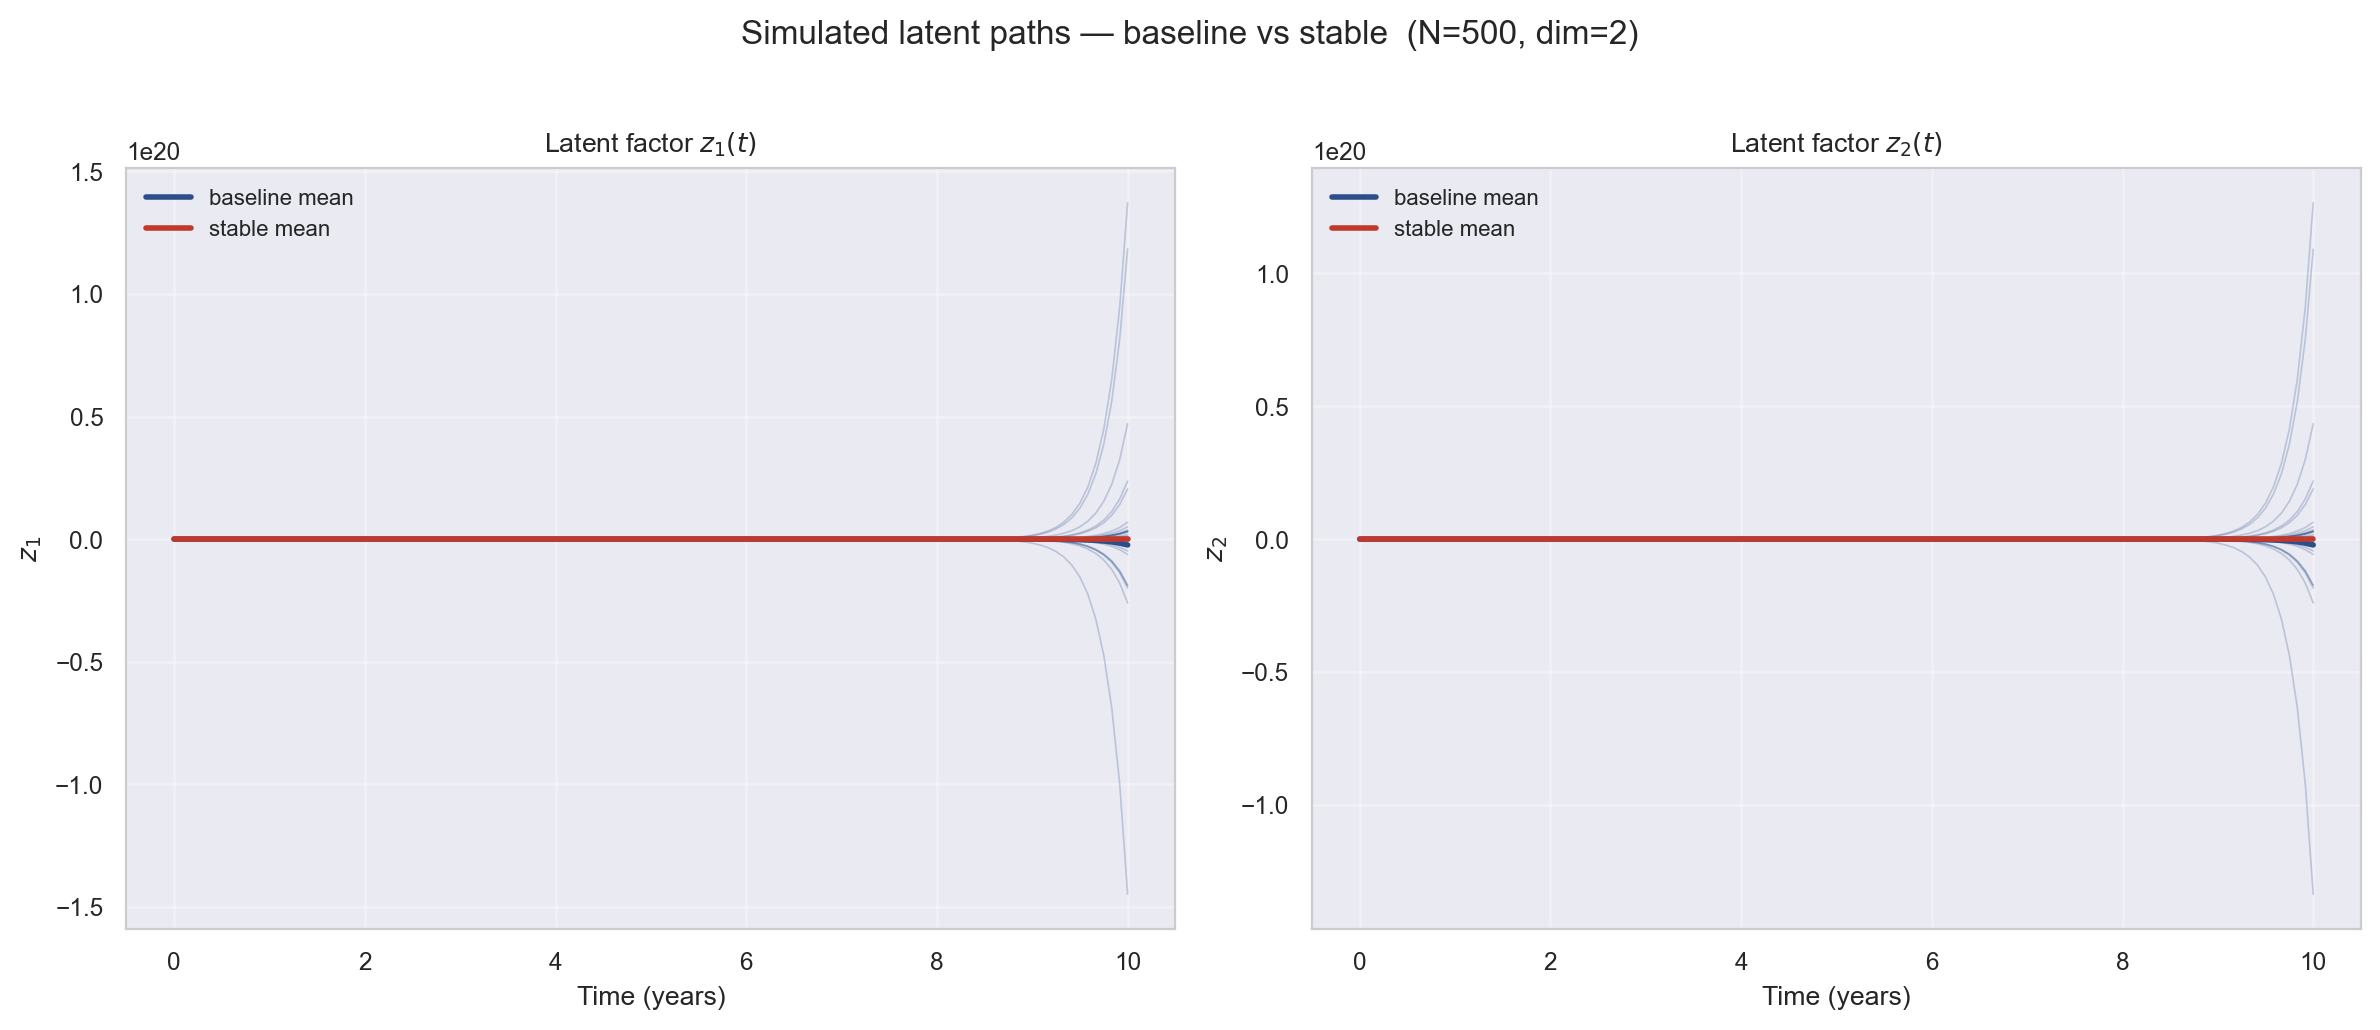
\includegraphics[width=\textwidth]{Figures/Pricing/ep3500_comparison/fig1_latent_paths.png}
    \caption{Individual Euler--Maruyama paths for $z_1(t)$ and $z_2(t)$ over 10 years
    ($N = 500$, 30 paths plotted).
    \textbf{Blue}: baseline ep3500. \textbf{Red}: stable ep3500.
    The baseline paths diverge to $|z| \sim 10^{20}$ within the simulation window,
    while the stable paths remain in the neighbourhood of the initial latent state
    and revert toward the model's equilibrium.}
    \label{fig:comp_latent_paths}
\end{figure}

The most immediate visual signal in Figure~\ref{fig:comp_latent_paths} is the
scale of the $y$-axis: the baseline paths (blue) occupy a range of order $10^{20}$
while the stable paths (red) stay within $[-3, +4]$, the natural support of the
training data.
This directly reflects the unstable eigenvalue(s) in the baseline drift matrix:
even with a $\Delta t = 1/12$ step, one positively aligned eigenvalue causes the
solution to grow exponentially at rate $\exp(\lambda_{\max} t)$, and after
120 steps $\lambda_{\max} > 0$ produces a divergent trajectory.

%--------------------------------------------------------
\subsection{Figure 2: Short rate paths}
\label{subsec:fig2}
%--------------------------------------------------------

\begin{figure}[H]
    \centering
    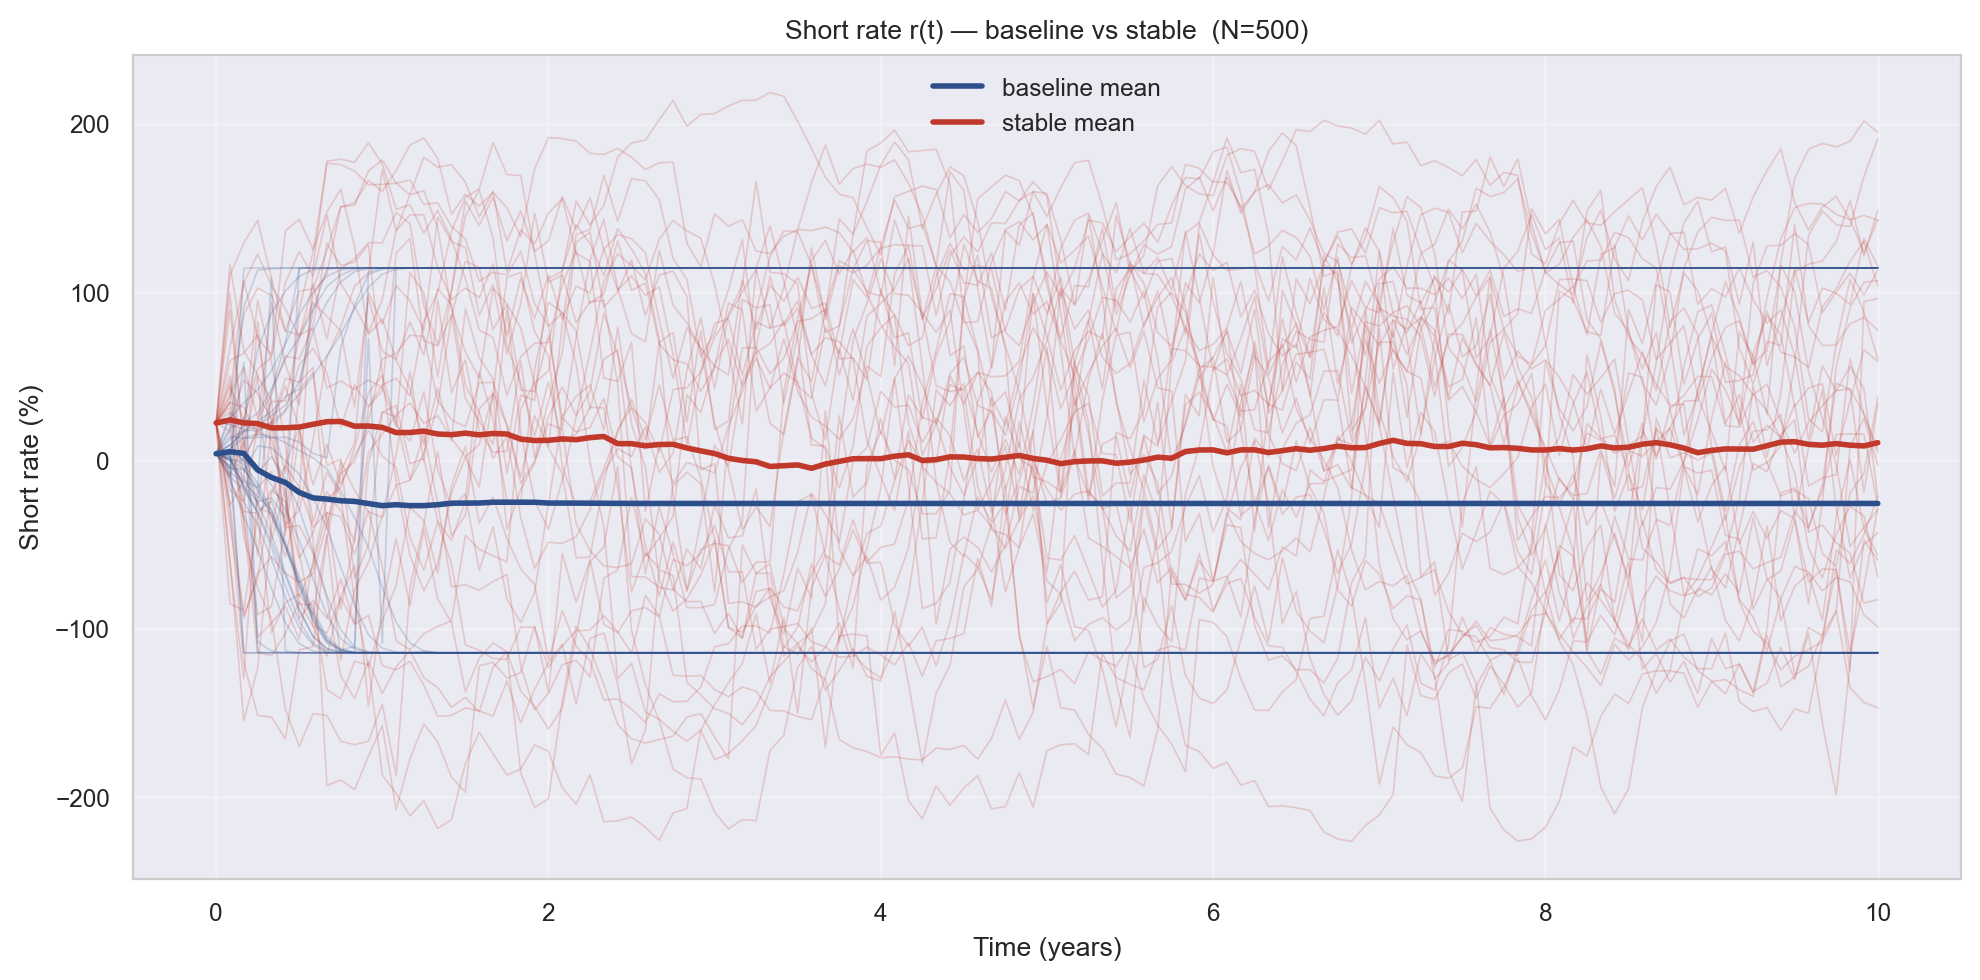
\includegraphics[width=\textwidth]{Figures/Pricing/ep3500_comparison/fig2_short_rate.png}
    \caption{Short-rate paths $r(t)$ over 10 years for both models.
    The baseline short rate (blue) immediately saturates at the hard limits of the
    centered soft-step output layer (bounded by $\pm\tfrac{1}{2}\|W_2\|_1$), while
    the stable short rate (red) evolves smoothly within
    an economically plausible range.}
    \label{fig:comp_short_rate_paths}
\end{figure}

Figure~\ref{fig:comp_short_rate_paths} shows the consequence of the divergent
latent state on the short rate.
Because $\tilde{r}(z) = W_2\,\psi(W_1 z)$ with $\psi\in(-\tfrac{1}{2},\tfrac{1}{2})$,
the output is bounded for any $z$, but once $\|z\|$ is large the centered soft-step
saturates component-wise at $\pm\tfrac{1}{2}$, pinning $\tilde{r}$ at
$\pm\tfrac{1}{2}\|W_2\|_1$.
All 500 baseline paths are immediately pinned to $\pm 114$\,bp and remain there
for the entire horizon.
The stable short rate, by contrast, starts near the initial observed level and
drifts within a roughly $\pm 2$\% band --- consistent with the EUR rate environment
of the training data.

%--------------------------------------------------------
\subsection{Figure 3: Terminal distributions}
\label{subsec:fig3}
%--------------------------------------------------------

\begin{figure}[H]
    \centering
    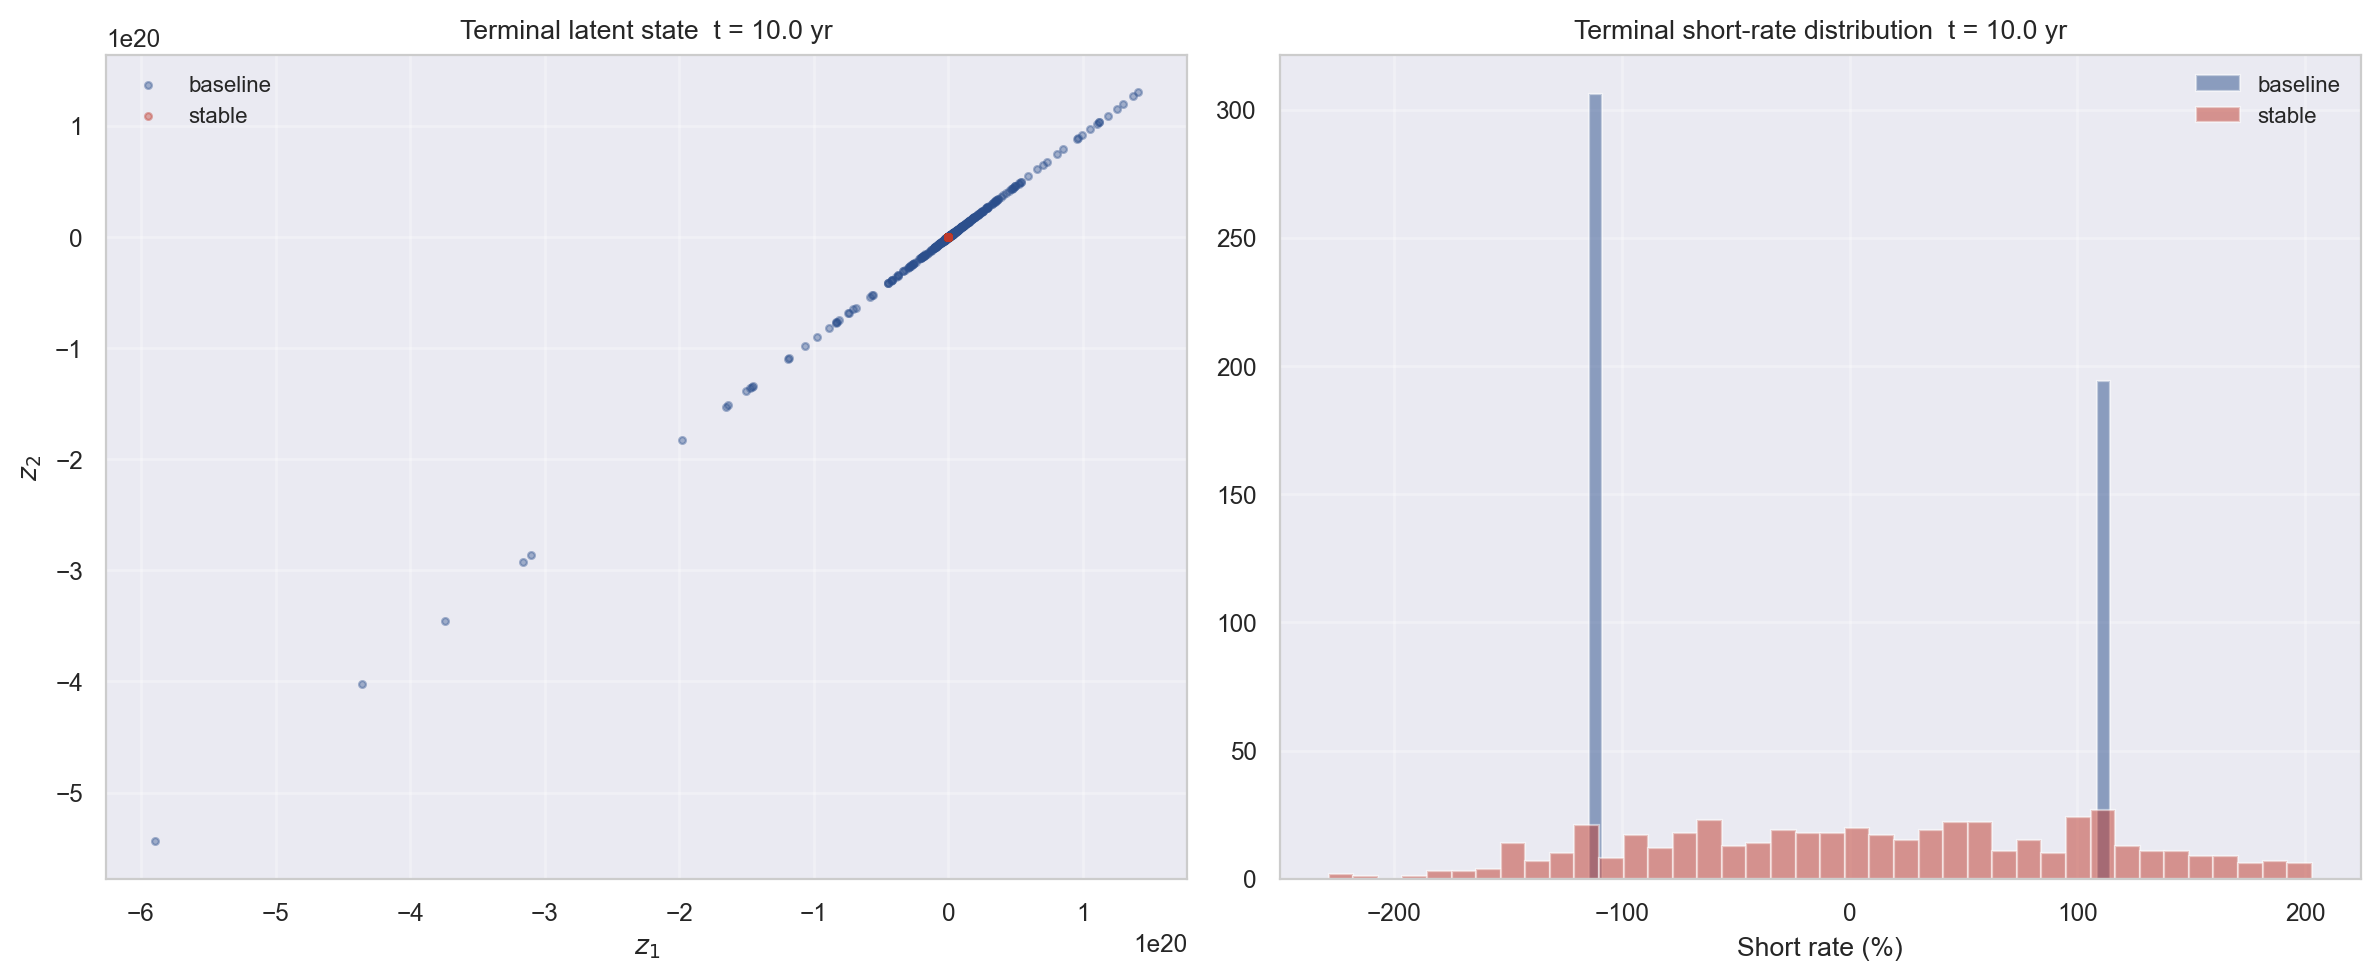
\includegraphics[width=\textwidth]{Figures/Pricing/ep3500_comparison/fig3_terminal_distributions.png}
    \caption{\textit{Left}: Terminal latent-state scatter plot at $t = 10$ yr
    for baseline (blue) and stable (red).
    \textit{Right}: Histogram of terminal short rates.
    The baseline terminal cloud is spread across an enormous region ($|z| \sim 10^{20}$);
    the stable terminal cloud occupies a compact region close to the initial point.}
    \label{fig:comp_terminal}
\end{figure}

Figure~\ref{fig:comp_terminal} (left) contrasts the terminal distributions of
$(z_1, z_2)$ at $t = 10$ yr.
The stable terminal cloud (red) forms a tight, well-centred ellipse that reflects
the mean-reversion of the Ornstein--Uhlenbeck-type dynamics --- paths diffuse away
from $z_0$ early on but are pulled back by the stable drift over time.
The baseline terminal cloud (blue) would occupy a region of radius $10^{20}$ and
is compressed to a single pixel on any reasonable axis scale.

The right panel confirms the short-rate saturation: the baseline produces a bimodal
distribution concentrated at $\pm 114$\,bp (the saturation limits of
the trained $W_2\,\psi(W_1 z)$ short-rate network), while the stable
model produces a unimodal, approximately Gaussian distribution.
The unimodal distribution is a direct consequence of mean-reversion: paths spend
most of the 10-year window near the equilibrium short rate rather than exploring
the tails.

%--------------------------------------------------------
\subsection{Figures 4--5: Percentile fan charts}
\label{subsec:figs45}
%--------------------------------------------------------

\begin{figure}[H]
    \centering
    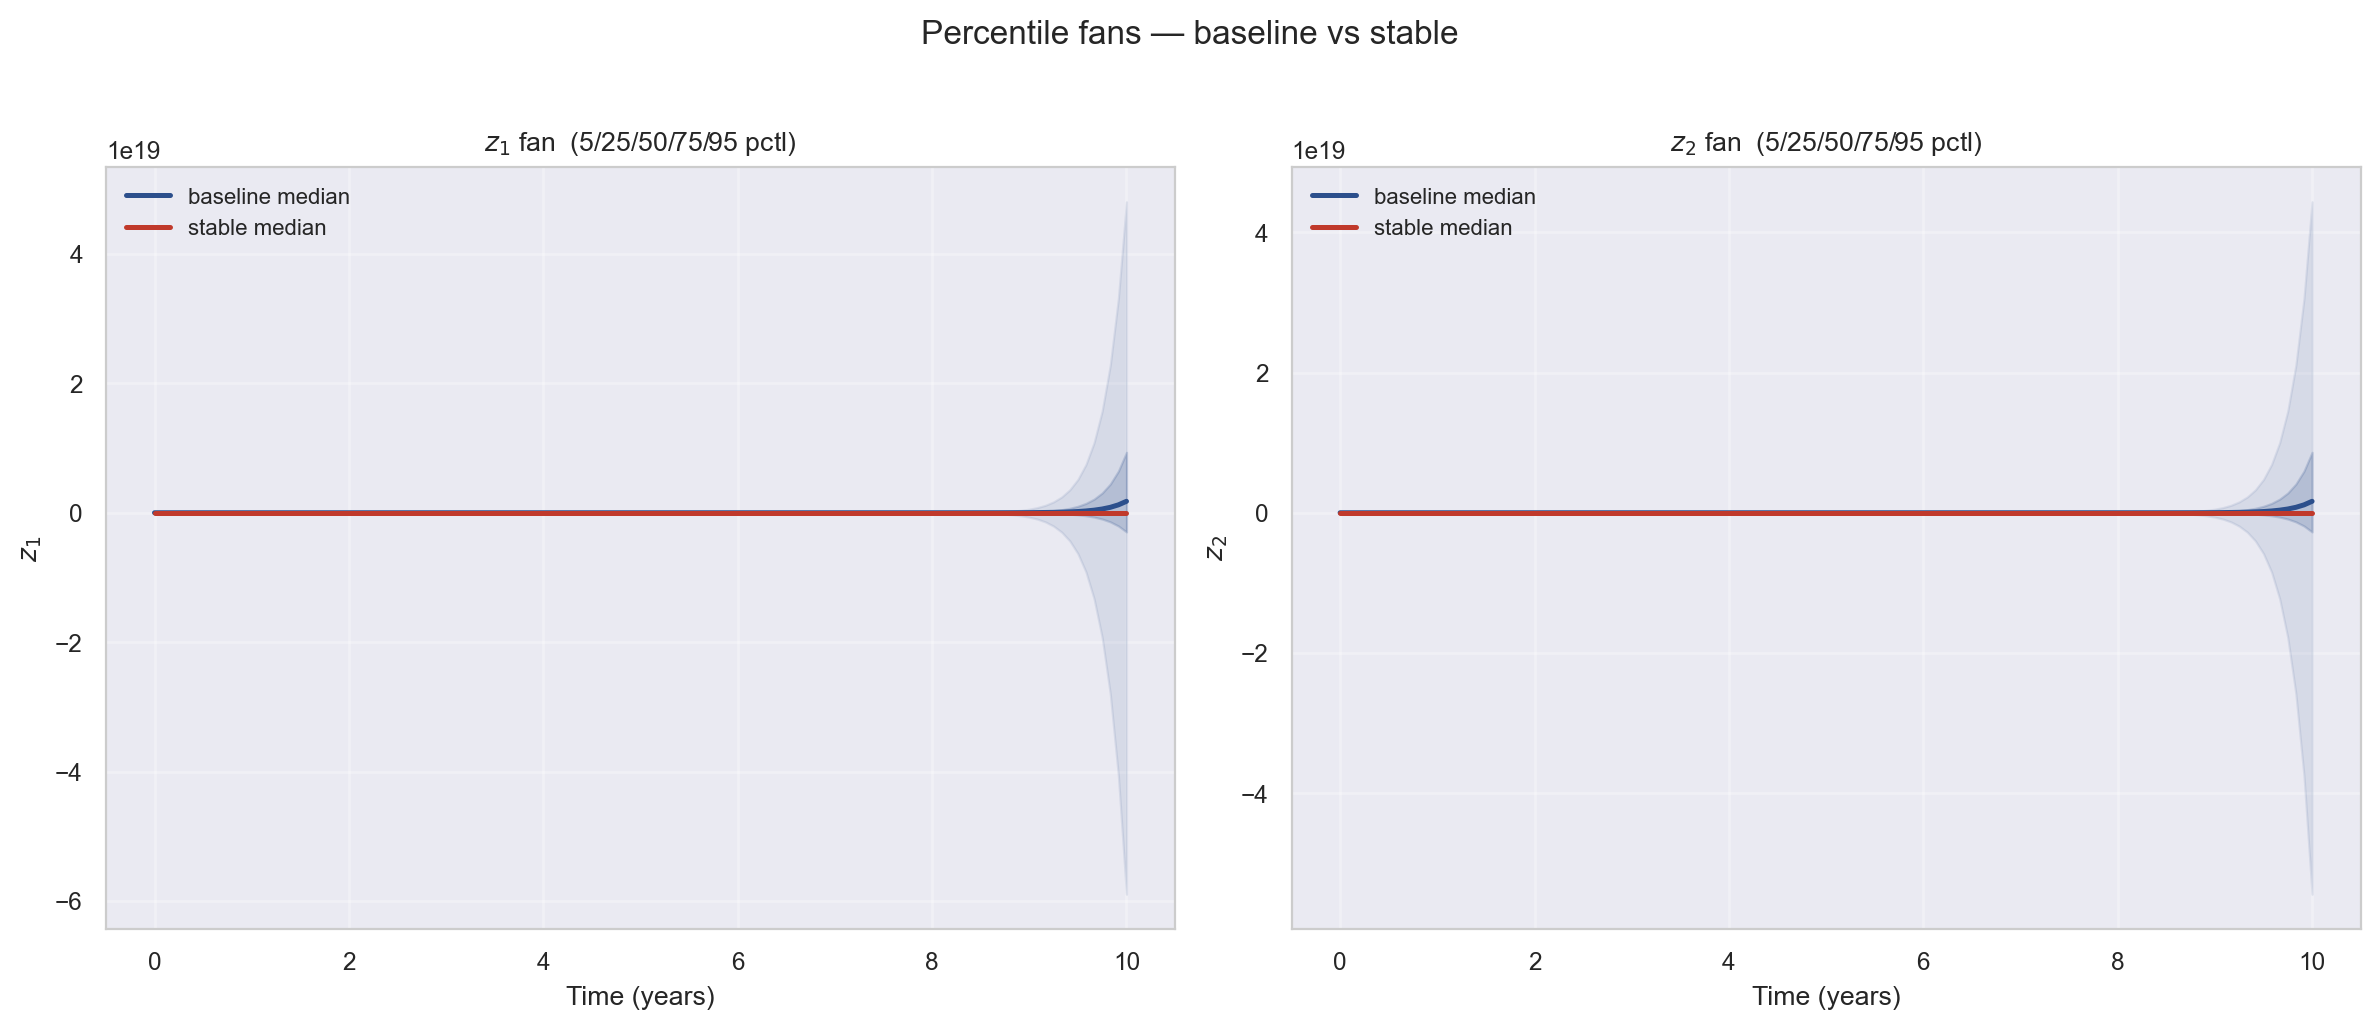
\includegraphics[width=\textwidth]{Figures/Pricing/ep3500_comparison/fig4_percentile_fans.png}
    \caption{Percentile fan charts for $z_1(t)$ (left) and $z_2(t)$ (right).
    Bands show the 5--95 and 25--75 percentile ranges across 500 paths.
    \textbf{Blue}: baseline. \textbf{Red}: stable.
    Solid lines show the median.
    The baseline fans diverge exponentially; the stable fans expand briefly and
    then stabilise as mean reversion dominates.}
    \label{fig:comp_fans}
\end{figure}

\begin{figure}[H]
    \centering
    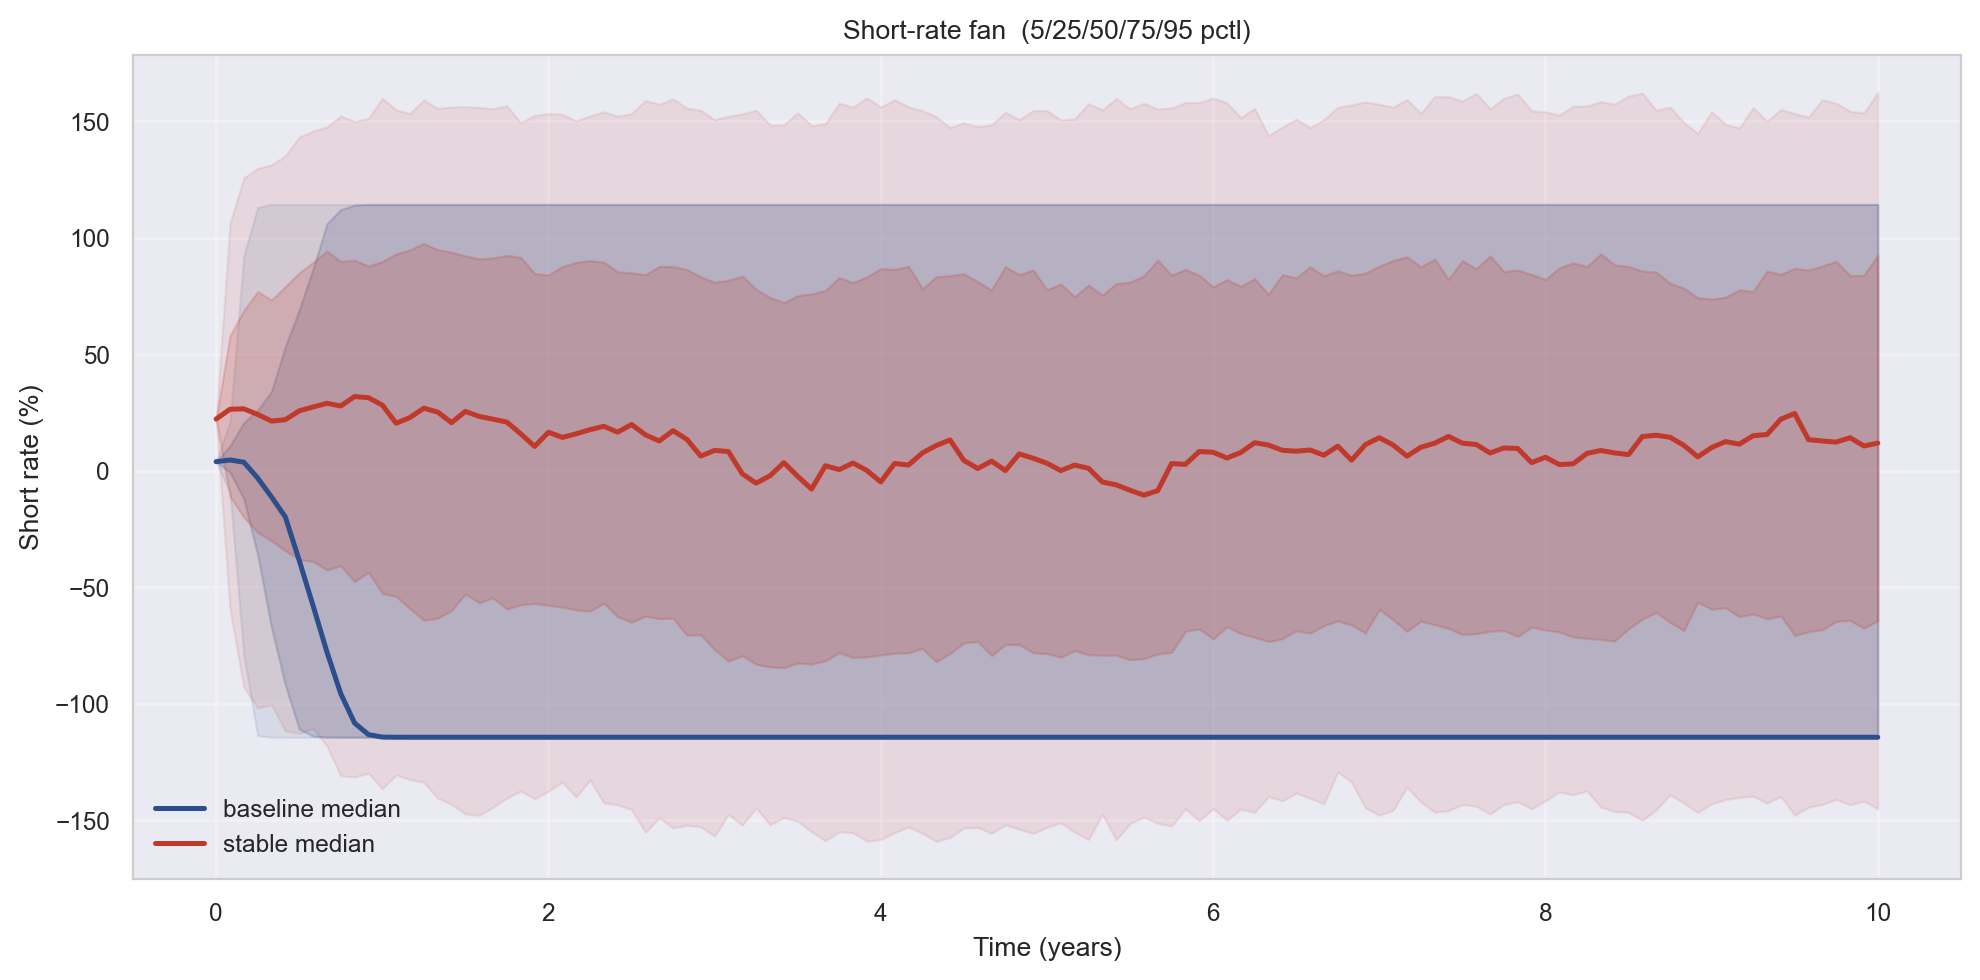
\includegraphics[width=\textwidth]{Figures/Pricing/ep3500_comparison/fig5_short_rate_fan.png}
    \caption{Short-rate percentile fan chart (5/25/50/75/95) for baseline (blue)
    and stable (red).
    The baseline fan immediately saturates and becomes flat; the stable fan
    evolves smoothly and narrows at longer horizons as mean reversion pulls all
    paths toward the equilibrium rate.}
    \label{fig:comp_short_rate_fan}
\end{figure}

Figures~\ref{fig:comp_fans} and~\ref{fig:comp_short_rate_fan} display the same
information in a summary form that is more informative for risk assessment.

For the \textbf{stable model} (red), the fan structure follows the
expected pattern of an Ornstein--Uhlenbeck process:
\begin{enumerate}
    \item \textit{Early diffusion phase} ($t \lesssim 1$\,yr): uncertainty grows
    as paths spread from the common starting point $z_0$.
    \item \textit{Mean-reversion phase} ($t \gtrsim 2$\,yr): the Hurwitz
    constraint pulls all paths toward $z^*$, and the bands stabilise or even
    narrow.
    The long-run distribution is the stationary distribution of the SDE,
    which is a Gaussian with covariance determined by the Lyapunov equation
    $M\Sigma_\infty + \Sigma_\infty M^\top + \Sigma(z^*)^2 = 0$.
\end{enumerate}

For the \textbf{baseline model} (blue), the fan structure is entirely different:
\begin{enumerate}
    \item The 5--95 band expands exponentially from the start, reflecting the
    positive eigenvalue(s) of $M$.
    \item The short-rate fan (Figure~\ref{fig:comp_short_rate_fan}, blue)
    is almost perfectly flat after the first time step: every path is saturated at
    $\pm r_{\mathrm{scale}}$ and the $50^{\mathrm{th}}$ percentile median
    oscillates near zero, reflecting an equal split between positively and
    negatively divergent paths.
\end{enumerate}

The qualitative contrast between the two sets of fans is exactly what the theory
predicts: stable means bounded uncertainty that grows and then stabilises;
baseline means unbounded uncertainty that grows without limit.


%========================================================
\section{Summary}
\label{sec:sim_summary}
%========================================================

Table~\ref{tab:sim_comparison_summary} summarises the key diagnostics.

\begin{table}[H]
\centering
\caption{Simulation diagnostics for baseline and stable ($\ell = 2$, ep3500,
EUR, $N = 500$ paths, $T = 10$\,yr, $\Delta t = 1/12$).
Short-rate values in basis points.}
\label{tab:sim_comparison_summary}
\begin{tabular}{@{}lrr@{}}
\toprule
\textbf{Metric} & \textbf{Baseline} & \textbf{Stable} \\
\midrule
$z_1$ mean at $T$      & $-6.3 \times 10^{16}$ & $-0.04$ \\
$z_1$ std over all $t$ & $6.8 \times 10^{18}$  & $0.61$  \\
$z_1$ range            & $[-5.9\times10^{20},\; 1.4\times10^{20}]$ & $[-2.38,\; 3.76]$ \\
\midrule
$z_2$ mean at $T$      & $-5.8 \times 10^{16}$ & $-0.29$ \\
$z_2$ std over all $t$ & $6.3 \times 10^{18}$  & $0.27$  \\
$z_2$ range            & $[-5.4\times10^{20},\; 1.3\times10^{20}]$ & $[-2.48,\; 0.49]$ \\
\midrule
$r$ mean (bp)          & $-24$ & $+8$   \\
$r$ std (bp)           & $109$ & $94$   \\
$r$ range (bp)         & $[-114,\; +114]$ & $[-233,\; +222]$ \\
All paths finite       & Yes (saturated) & Yes (well-behaved) \\
Paths usable for pricing & \textbf{No} & \textbf{Yes} \\
\bottomrule
\end{tabular}
\end{table}

The central conclusion is that the three structural constraints introduced by
the stable parameterization --- Hurwitz drift, sigmoid-bounded volatilities, and
hyperspherical positive-definite correlations --- are not merely theoretical
niceties.
They are \emph{necessary} for the model to produce paths that are usable for
simulation-based derivative pricing.
The baseline model, despite fitting the training data equally well
(comparable in-sample and out-of-sample reconstruction errors; see
Chapter~\ref{chap:results_stable}), is entirely unusable as a pricing engine
once $t > 0$.

The stable ep3500 checkpoint therefore serves as the natural starting point for
the second-stage pricing calibration developed in the following chapter on
simulation-based derivative pricing.

